\documentclass[10pt,twocolumn]{article}
\usepackage[utf8]{inputenc}
\usepackage[margin=0.75in]{geometry}
\usepackage{graphicx}
\usepackage{amsmath}
\usepackage{listings}
\usepackage{xcolor}
\usepackage{hyperref}
\usepackage{tikz}
\usepackage{pgfplots}
\usepackage{float}
\usepackage{caption}
\usepackage{multirow}
\usepackage{booktabs}
\usepackage{titlesec}

\usetikzlibrary{shapes.geometric, arrows.meta, positioning, calc, shadows, decorations.pathreplacing, fit, backgrounds}

% Code listing style
\lstdefinestyle{cpp}{
    language=C++,
    basicstyle=\ttfamily\footnotesize,
    keywordstyle=\color{blue}\bfseries,
    commentstyle=\color{green!60!black}\itshape,
    stringstyle=\color{red},
    numbers=left,
    numberstyle=\tiny\color{gray},
    frame=single,
    breaklines=true,
    captionpos=b,
    tabsize=2
}

\hypersetup{
    colorlinks=true,
    linkcolor=blue,
    filecolor=magenta,
    urlcolor=cyan,
    citecolor=blue
}

\pgfplotsset{compat=1.18}

% Title formatting
\titleformat{\section}{\large\bfseries}{\thesection}{1em}{}
\titleformat{\subsection}{\normalsize\bfseries}{\thesubsection}{1em}{}
\titleformat{\subsubsection}{\small\bfseries}{\thesubsubsection}{1em}{}

\begin{document}

\twocolumn[
\begin{@twocolumnfalse}
\begin{center}
\LARGE\textbf{Fern: A Pedagogical Cross-Platform UI Framework\\Demonstrating Object-Oriented Design Principles\\Through Manual Pixel-Level Rendering}

\vspace{0.5cm}

\large Rishi Ahuja\\
\normalsize Object-Oriented Programming ITDC0201\\
Department of Information Technology\\
\texttt{rishia.it.24@nitj.ac.in}

\vspace{0.5cm}
\end{center}

\begin{abstract}
\noindent Modern UI frameworks abstract away the underlying rendering mechanics, leaving developers with limited understanding of how graphical user interfaces actually function at the foundational level. This paper presents \textbf{Fern}, an educational cross-platform UI framework implemented in C++17 that demonstrates core object-oriented programming (OOP) principles—encapsulation, inheritance, polymorphism, and abstraction—through a complete pixel-level rendering engine built entirely from scratch. Unlike conventional frameworks that rely on existing graphics libraries (OpenGL, DirectX, WebGL), Fern manually computes and renders every pixel, providing transparent insight into UI mechanics while maintaining a clean, declarative API inspired by modern frameworks like Flutter. The framework comprises approximately 12,000 lines of production-quality C++ code, featuring a hierarchical widget system, signal-slot event handling, responsive layout engine, and platform abstraction layer supporting native Linux (X11) and Web (WebAssembly) deployments. Fern integrates with a comprehensive development toolchain—the FernKit ecosystem—including Terra CLI for project management, Gleeb LSP for intelligent IDE support, and Conduit for network communication. Through this implementation, we demonstrate how fundamental OOP concepts enable the construction of complex, maintainable software systems while solving the real-world problem of rapid UI prototyping for educational and experimental applications.
\end{abstract}

\vspace{0.5cm}
\end{@twocolumnfalse}
]

\vspace{0.5cm}
\end{@twocolumnfalse}

\section{Introduction}

\subsection{Motivation and Context}

The modern software development landscape presents a curious paradox: while graphical user interfaces have become ubiquitous, understanding their fundamental mechanics has become increasingly rare. Contemporary UI frameworks—from web-based React and Vue to mobile frameworks like SwiftUI and Flutter—provide powerful abstractions that enable developers to create sophisticated interfaces with minimal code. However, this convenience comes at a pedagogical cost.

Students and developers rarely encounter questions like: How does a pixel actually appear on screen? What happens when you click a button? How does a layout algorithm determine where widgets should be positioned? These foundational concepts are hidden behind layers of abstraction, treated as implementation details rather than core knowledge. While this approach accelerates development, it creates a generation of developers who understand what UI frameworks do, but not how they work.

Simultaneously, the prototyping landscape faces its own challenge. When building experimental applications, educational tools, or quick visualizations, developers must choose between heavyweight solutions (Qt, GTK, comprehensive game engines) that bring extensive dependencies and complex build systems, or minimal solutions that lack the structure needed for maintainable code. The gap between "quick-and-dirty script" and "production-ready application" is vast, leaving little middle ground for educational exploration and rapid experimentation.

\subsection{Problem Definition}

This project addresses a dual challenge that sits at the intersection of education and practical software engineering:

\textbf{The Educational Problem:} Computer science education emphasizes algorithms, data structures, and design patterns, but rarely connects these concepts to tangible, visual outcomes. Students learn about inheritance and polymorphism through abstract examples (shapes, animals, vehicles) without seeing how these principles enable real systems. The question becomes: how can we create a framework that makes software architecture principles visible and comprehensible while remaining practically useful?

\textbf{The Practical Problem:} Rapid prototyping requires speed, but speed often requires infrastructure. Creating a particle physics simulation, an interactive data visualization, or an experimental interface concept shouldn't require days of dependency management, build configuration, and boilerplate code. The challenge is providing enough structure to write maintainable code without the friction of heavyweight frameworks.

Fern emerges as a response to both challenges. By implementing a complete UI framework from first principles—rendering every pixel manually, implementing every algorithm explicitly, and documenting every design decision—it serves simultaneously as an educational resource and a practical tool for rapid prototyping.

\subsection{Core Contributions}

This work makes five primary contributions to the understanding and application of object-oriented programming principles in systems design:

\textbf{1. Architectural Demonstration:} We present a complete, working system that explicitly demonstrates all four pillars of OOP—encapsulation, inheritance, polymorphism, and abstraction—not as isolated examples but as integrated components of a cohesive architecture. Each design decision is documented and justified, making the codebase itself a learning resource.

\textbf{2. Manual Rendering Pipeline:} The framework implements pixel-level graphics algorithms (Bresenham's line algorithm, circle rasterization, polygon filling) without any external graphics libraries, making every rendering decision transparent and modifiable. This transparency serves both educational goals (students can read and understand the algorithms) and practical goals (developers can modify rendering behavior for specific needs).

\textbf{3. Hierarchical Widget System:} We demonstrate the Composite design pattern through a complete widget hierarchy spanning 15+ components, from basic primitives (circles, lines, text) to complex containers (dropdowns, sliders, progress bars) and flexible layouts (rows, columns, responsive centering). The system shows how composition enables building complex UIs from simple, reusable components.

\textbf{4. Platform Abstraction:} Through the Strategy pattern, we achieve true platform independence, compiling the same codebase to native Linux applications (via X11) and web applications (via WebAssembly) without conditional compilation or platform-specific code in user applications.

\textbf{5. Educational Resource:} Beyond the implementation itself, the project includes comprehensive documentation (25+ pages), architectural diagrams, and working examples that make OOP principles concrete and understandable. The 12,000 lines of code serve as an extended case study in software architecture.

\section{Related Work and Positioning}

\subsection{UI Framework Evolution}

The evolution of UI frameworks reflects a continuous tension between power and complexity, between control and convenience. Early frameworks like Xt and Motif on Unix systems provided low-level access but required extensive code for simple interfaces. The Object-Oriented GUI revolution of the 1990s brought frameworks like MFC, Qt, and GTK, which introduced widget hierarchies and event-driven programming. These frameworks demonstrated how OOP principles could structure complex UI systems, but they abstracted away rendering details, relying on platform-native drawing APIs.

Modern frameworks have further increased abstraction levels. React's virtual DOM, Flutter's widget tree, and SwiftUI's declarative syntax enable developers to describe interfaces without concerning themselves with rendering mechanics. While this approach maximizes productivity, it minimizes understanding. Developers learn to use these frameworks without understanding the principles that make them work.

Fern positions itself deliberately in opposition to this trend. Rather than adding another layer of abstraction, it removes layers, exposing the foundational mechanics while maintaining a modern, ergonomic API. This approach aligns with frameworks like Processing and p5.js, which make graphics programming accessible for creative coding, but Fern extends the concept to complete UI development with proper software architecture.

\subsection{Educational Graphics Systems}

Several notable projects have attempted to make graphics programming more accessible. Processing, created by Ben Fry and Casey Reas, provides a simplified Java environment for creative coding, abstracting OpenGL while exposing drawing primitives. Its web counterpart, p5.js, brings these concepts to JavaScript and HTML5 Canvas. Raylib offers a simple C library for game programming, wrapping OpenGL but maintaining relatively low-level control.

These systems share Fern's educational goals but differ in approach. Processing and p5.js still rely on underlying graphics libraries (Java2D, OpenGL, HTML5 Canvas), abstracting rather than implementing rendering. Raylib provides more control but requires understanding OpenGL concepts. None of these systems implements rendering entirely in software, making algorithmic decisions invisible.

Fern's unique contribution is implementing every pixel operation explicitly in portable C++ code, compiled to both native and WebAssembly targets. Students can read the circle-drawing algorithm, modify it, understand why it works, and see their changes immediately reflected in running applications.

\section{System Architecture}

\subsection{Architectural Philosophy}

The architecture of Fern embodies a specific philosophy: complexity should be managed through layers, each layer should solve one problem well, and dependencies should flow in only one direction. This layered architecture serves multiple purposes: it makes the system understandable (each layer can be studied in isolation), testable (layers can be unit-tested independently), and extensible (new functionality can be added without modifying existing layers).

The system consists of five distinct layers, each with clearly defined responsibilities and interfaces. Upper layers depend on lower layers, but not vice versa, creating a directed acyclic graph of dependencies that prevents circular coupling. This structure is not just good software engineering—it's pedagogically valuable, allowing students to understand the system bottom-up or top-down depending on their learning style.

\subsection{Complete System Architecture}

Figure \ref{fig:complete-arch} presents the complete system architecture, showing how data flows from user code through the widget system, into the core management layer, down to graphics primitives, and finally to platform-specific rendering. This diagram represents the actual runtime architecture, not an idealized design document—every arrow corresponds to real method calls in the implementation.

\begin{figure*}[t]
\centering
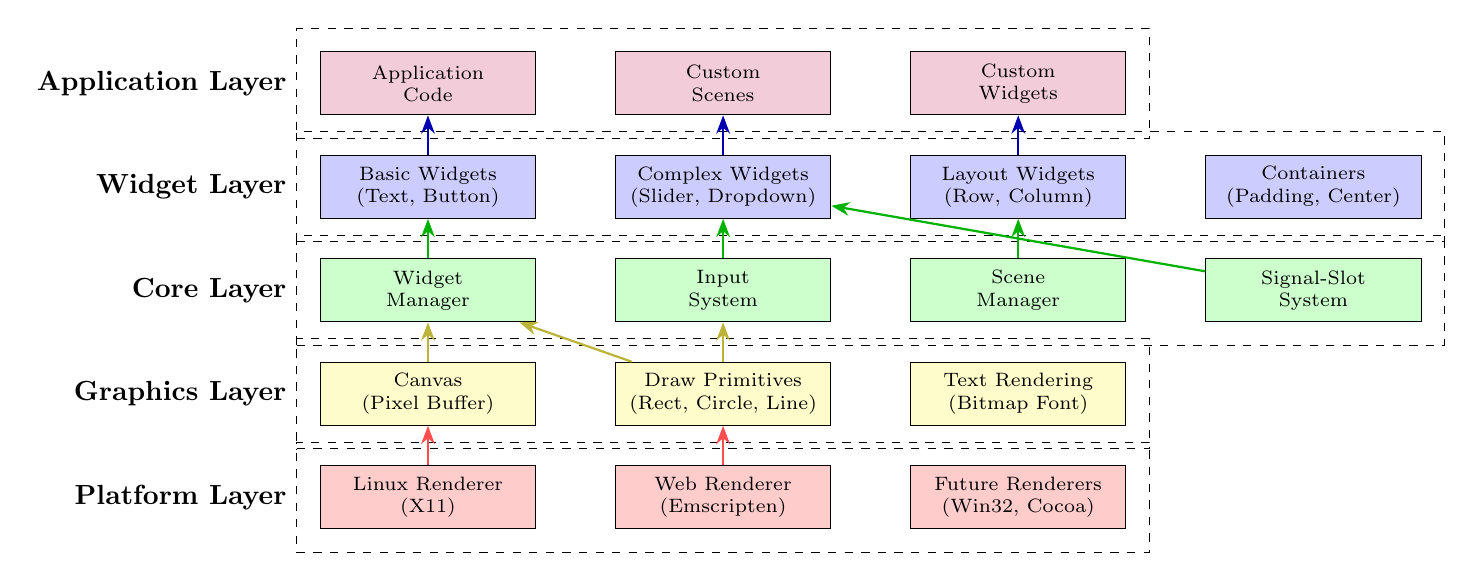
\begin{tikzpicture}[
    node distance=0.5cm and 1cm,
    box/.style={rectangle, draw, text width=2.5cm, minimum height=0.8cm, align=center, font=\scriptsize},
    layer/.style={rectangle, draw, dashed, inner sep=0.3cm},
    arrow/.style={-Stealth, thick},
]

% Platform Layer (Bottom)
\begin{scope}[local bounding box=platform]
    \node[box, fill=red!20] (linux) {Linux Renderer\\(X11)};
    \node[box, fill=red!20, right=of linux] (web) {Web Renderer\\(Emscripten)};
    \node[box, fill=red!20, right=of web] (future) {Future Renderers\\(Win32, Cocoa)};
\end{scope}
\node[layer, fit=(platform), label=left:\textbf{Platform Layer}] {};

% Graphics Layer
\begin{scope}[local bounding box=graphics, yshift=2cm]
    \node[box, fill=yellow!20, above=of linux] (canvas) {Canvas\\(Pixel Buffer)};
    \node[box, fill=yellow!20, above=of web] (primitives) {Draw Primitives\\(Rect, Circle, Line)};
    \node[box, fill=yellow!20, above=of future] (text) {Text Rendering\\(Bitmap Font)};
\end{scope}
\node[layer, fit=(graphics), label=left:\textbf{Graphics Layer}] {};

% Core Layer
\begin{scope}[local bounding box=core, yshift=4cm]
    \node[box, fill=green!20, above=of canvas] (widgetmgr) {Widget\\Manager};
    \node[box, fill=green!20, above=of primitives] (input) {Input\\System};
    \node[box, fill=green!20, above=of text] (scene) {Scene\\Manager};
    \node[box, fill=green!20, right=of scene] (signal) {Signal-Slot\\System};
\end{scope}
\node[layer, fit=(core), label=left:\textbf{Core Layer}] {};

% Widget Layer
\begin{scope}[local bounding box=widgets, yshift=6cm]
    \node[box, fill=blue!20, above=of widgetmgr] (basic) {Basic Widgets\\(Text, Button)};
    \node[box, fill=blue!20, above=of input] (complex) {Complex Widgets\\(Slider, Dropdown)};
    \node[box, fill=blue!20, above=of scene] (layout) {Layout Widgets\\(Row, Column)};
    \node[box, fill=blue!20, above=of signal] (container) {Containers\\(Padding, Center)};
\end{scope}
\node[layer, fit=(widgets), label=left:\textbf{Widget Layer}] {};

% Application Layer
\begin{scope}[local bounding box=app, yshift=8cm]
    \node[box, fill=purple!20, above=of basic] (usercode1) {Application\\Code};
    \node[box, fill=purple!20, above=of complex] (usercode2) {Custom\\Scenes};
    \node[box, fill=purple!20, above=of layout] (usercode3) {Custom\\Widgets};
\end{scope}
\node[layer, fit=(app), label=left:\textbf{Application Layer}] {};

% Arrows showing data flow
\draw[arrow, red!70] (linux) -- (canvas);
\draw[arrow, red!70] (web) -- (primitives);
\draw[arrow, yellow!70!black] (canvas) -- (widgetmgr);
\draw[arrow, yellow!70!black] (primitives) -- (widgetmgr);
\draw[arrow, yellow!70!black] (primitives) -- (input);
\draw[arrow, green!70!black] (widgetmgr) -- (basic);
\draw[arrow, green!70!black] (input) -- (complex);
\draw[arrow, green!70!black] (scene) -- (layout);
\draw[arrow, green!70!black] (signal) -- (complex);
\draw[arrow, blue!70!black] (basic) -- (usercode1);
\draw[arrow, blue!70!black] (complex) -- (usercode2);
\draw[arrow, blue!70!black] (layout) -- (usercode3);

\end{tikzpicture}
\caption{Complete Fern architecture showing all five layers and their interactions. Arrows indicate dependency direction—upper layers call into lower layers, never the reverse. This strict layering enables independent testing and modification of each layer.}
\label{fig:complete-arch}
\end{figure*}

At the foundation sits the \textbf{Platform Layer}, which abstracts operating system specifics. This layer handles window creation, event polling, and display management. The key insight here is polymorphism: the main application loop operates on a \texttt{PlatformRenderer} interface, and concrete implementations (LinuxRenderer, WebRenderer) handle platform-specific details. This design enables true platform independence—the same application binary (when compiled to WebAssembly) runs in web browsers without modification.

Above this sits the \textbf{Graphics Layer}, which provides pixel-level rendering operations. The \texttt{Canvas} class manages the pixel buffer—a contiguous array of 32-bit RGBA values. The \texttt{Draw} namespace implements geometric primitives (rectangles, circles, lines) using classical algorithms. This layer demonstrates encapsulation: the pixel buffer is never accessed directly; all operations go through controlled interfaces with automatic bounds checking.

The \textbf{Core Layer} manages application-level concerns. The \texttt{WidgetManager} maintains the collection of active widgets, handling their lifecycle, rendering order, and input distribution. The \texttt{Input} system normalizes platform-specific events into a uniform \texttt{InputState} structure. The \texttt{SceneManager} implements stack-based navigation for multi-screen applications. The \texttt{Signal-Slot} system provides type-safe event callbacks. This layer demonstrates the Singleton and Observer patterns.

The \textbf{Widget Layer} implements reusable UI components through inheritance from a base \texttt{Widget} class. Simple widgets like \texttt{TextWidget} and \texttt{CircleWidget} render themselves directly using the Graphics Layer. Complex widgets like \texttt{ButtonWidget} and \texttt{SliderWidget} incorporate state management and event handling. Layout widgets like \texttt{RowWidget} and \texttt{ColumnWidget} implement positioning algorithms. This layer demonstrates the Composite pattern and inheritance hierarchies.

Finally, the \textbf{Application Layer} represents user code that composes widgets into complete interfaces. Applications instantiate widgets, connect signal handlers, and implement custom rendering logic. This separation of concerns means application developers work with high-level abstractions while the framework handles low-level details.

\subsection{Data Flow and Execution Model}

Understanding the runtime behavior requires following data as it flows through the system. Consider a single frame of execution:

\textbf{Step 1: Event Collection.} The platform layer polls for OS events (mouse movements, key presses, window resizes). These events are converted to normalized format and passed to the Input system.

\textbf{Step 2: Input Distribution.} The WidgetManager receives the current InputState and distributes it to widgets in reverse Z-order (top widgets first). Each widget's \texttt{handleInput()} method returns true if it consumed the event, preventing underlying widgets from processing it.

\textbf{Step 3: State Updates.} Widgets update their internal state based on input. Buttons change their visual state (normal, hovered, pressed). Text inputs append characters to their buffers. Sliders recalculate their values based on mouse position.

\textbf{Step 4: Signal Emission.} Widgets that have experienced significant state changes emit signals. A button emits \texttt{onClick} when clicked. A slider emits \texttt{onValueChanged} when dragged. Application code listening to these signals executes callback functions.

\textbf{Step 5: Rendering.} The application's draw callback executes, typically calling \texttt{Draw::fill()} to clear the screen. The WidgetManager then calls \texttt{render()} on each widget in forward Z-order (back widgets first). Each widget uses Graphics Layer primitives to draw itself onto the canvas.

\textbf{Step 6: Presentation.} The complete frame buffer is passed to the platform layer's \texttt{present()} method, which transfers pixels to the display. On Linux, this involves XPutImage to X11. On web, it involves JavaScript interop to write to HTML5 Canvas.

This cycle repeats 60 times per second (or as fast as the system allows), creating the illusion of interactivity. The clean separation of concerns means each step can be understood, debugged, and optimized independently.

\section{Object-Oriented Principles in Practice}

This section examines how the four pillars of object-oriented programming manifest in Fern's architecture. Rather than presenting these principles as abstract concepts, we show their practical application in solving real software engineering challenges.

\subsection{Encapsulation: Information Hiding and Interface Design}

Encapsulation—the bundling of data with methods that operate on that data, while restricting direct access to internal state—serves as Fern's first line of defense against complexity. Every major component demonstrates this principle at different granularities.

\subsubsection{Canvas Encapsulation}

The \texttt{Canvas} class exemplifies encapsulation at the data structure level. It manages a pixel buffer—a raw array of millions of 32-bit integers—but exposes this complex resource through a simple, safe interface:

\begin{lstlisting}[style=cpp, basicstyle=\ttfamily\tiny]
class Canvas {
public:
    void clear(uint32_t color);
    void setPixel(int x, int y, uint32_t color);
    uint32_t getPixel(int x, int y) const;
private:
    uint32_t* buffer_;  // Hidden
    int width_, height_; // Hidden
};
\end{lstlisting}

Why does this matter? Consider the consequences of direct buffer access: clients could write out-of-bounds, causing memory corruption; they could forget to account for row stride, writing pixels to wrong locations; they could access the buffer from multiple threads without synchronization. By encapsulating the buffer behind \texttt{setPixel()}, we add automatic bounds checking, enforce single-threaded access, and maintain the freedom to change internal representation (perhaps switching to a tile-based structure) without affecting client code.

This design also demonstrates const-correctness—\texttt{getPixel()} is marked const, enabling the compiler to enforce read-only access and enabling optimization. Students studying this code see how language features (const, private) enable robust software design.

\subsubsection{Input State Management}

The \texttt{Input} class encapsulates global input state, addressing a classic software engineering problem: how do you manage shared mutable state safely? The answer: you don't share it—you encapsulate it.

Platform-specific code updates input through dedicated methods (\texttt{updateMousePosition()}, \texttt{updateKeyPress()}), while widgets read through \texttt{getState()}, which returns a const reference. This asymmetric interface prevents widgets from accidentally modifying input state, eliminating a entire class of bugs. At frame boundaries, \texttt{resetEvents()} clears frame-specific flags (like \texttt{mouseClicked}), ensuring events don't persist across frames.

The educational value here is profound: students see how careful interface design eliminates bugs before they can occur, not through testing but through structure.

\subsection{Inheritance: Code Reuse Through Hierarchies}

Inheritance enables both interface specification (through abstract base classes) and implementation sharing (through concrete base classes). Fern uses both extensively, demonstrating when each approach is appropriate.

\subsubsection{Widget Hierarchy Design}

The widget hierarchy (Figure \ref{fig:widget-hierarchy}) demonstrates inheritance for interface definition. All UI components inherit from abstract \texttt{Widget}:


\begin{figure*}[t]
\centering
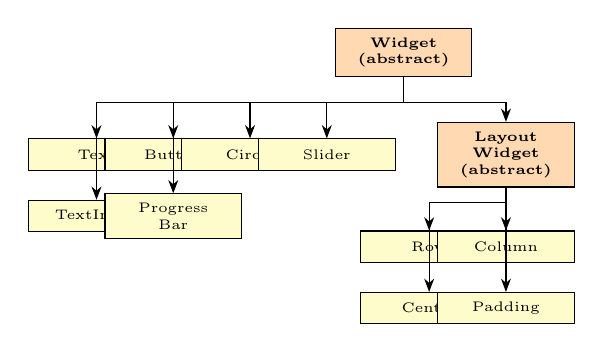
\begin{tikzpicture}[
    scale=0.65,
    node distance=0.8cm and 1cm,
    class/.style={rectangle, draw, fill=yellow!20, text width=1.5cm, minimum height=0.4cm, align=center, font=\tiny},
    abstract/.style={rectangle, draw, fill=orange!30, text width=1.5cm, minimum height=0.4cm, align=center, font=\tiny\bfseries},
    arrow/.style={-Stealth, thin}
]
% Base - Widget (centered at top)
\node[abstract] (widget) at (0,0) {Widget\\(abstract)};

% Level 1 - All direct children of Widget at same vertical level
% Left side: concrete widgets in a row
\node[class] (text) at (-6,-2) {Text};
\node[class] (button) at (-4.5,-2) {Button};
\node[class] (circle) at (-3,-2) {Circle};
\node[class] (slider) at (-1.5,-2) {Slider};
\node[class] (input) at (-6,-3.2) {TextInput};
\node[class] (progress) at (-4.5,-3.2) {Progress\\Bar};

% Right side: LayoutWidget (abstract, same level as other children)
\node[abstract] (layout) at (2,-2) {Layout\\Widget\\(abstract)};

% Level 2 - Layout descendants (children of LayoutWidget only)
\node[class] (row) at (0.5,-3.8) {Row};
\node[class] (column) at (2,-3.8) {Column};
\node[class] (center) at (0.5,-5) {Center};
\node[class] (padding) at (2,-5) {Padding};

% Arrows from Widget to ALL its direct children
\draw[arrow] (widget.south) -- ++(0,-0.5) -| (text.north);
\draw[arrow] (widget.south) -- ++(0,-0.5) -| (button.north);
\draw[arrow] (widget.south) -- ++(0,-0.5) -| (circle.north);
\draw[arrow] (widget.south) -- ++(0,-0.5) -| (slider.north);
\draw[arrow] (widget.south) -- ++(0,-0.5) -| (input.north);
\draw[arrow] (widget.south) -- ++(0,-0.5) -| (progress.north);
\draw[arrow] (widget.south) -- ++(0,-0.5) -| (layout.north);

% Arrows from LayoutWidget to its children only
\draw[arrow] (layout.south) -- ++(0,-0.3) -| (row.north);
\draw[arrow] (layout.south) -- ++(0,-0.3) -| (column.north);
\draw[arrow] (layout.south) -- ++(0,-0.3) -| (center.north);
\draw[arrow] (layout.south) -- ++(0,-0.3) -| (padding.north);
\end{tikzpicture}
\caption{Complete widget class hierarchy showing 15+ concrete widgets inheriting from abstract base. LayoutWidget provides intermediate abstraction for container widgets. All widgets implement render() and handleInput() virtual methods, enabling polymorphic collections in WidgetManager.}
\label{fig:widget-hierarchy}
\end{figure*}


The base \texttt{Widget} defines pure virtual methods (\texttt{render()}, \texttt{handleInput()}) that derived classes must implement. This approach creates a contract: anything that inherits from Widget can be rendered and can handle input. The WidgetManager exploits this property, storing heterogeneous widgets in a single container and treating them uniformly.

But Widget also provides concrete functionality—position and size management through protected members (\texttt{x\_}, \texttt{y\_}, \texttt{width\_}, \texttt{height\_}). Every widget needs these properties, so the base class provides them, demonstrating implementation inheritance. Derived classes access these through protected visibility, enabling sharing without exposing them to external clients.

\subsubsection{Platform Abstraction Through Inheritance}

Platform-specific code demonstrates inheritance for polymorphism. The \texttt{PlatformRenderer} interface defines operations all platforms must support, while \texttt{LinuxRenderer} and \texttt{WebRenderer} provide platform-specific implementations. The main loop operates on \texttt{PlatformRenderer*}, achieving platform independence through virtual dispatch.

This design makes adding new platforms straightforward: implement the interface, register the factory, recompile. No changes to existing code required. Students learn that good abstraction enables extension without modification—a core principle of sustainable software design.

\subsection{Polymorphism: Uniform Interfaces, Diverse Implementations}

Polymorphism enables treating different types uniformly, writing code that operates on abstractions rather than concrete types. Fern demonstrates both runtime (virtual functions) and compile-time (templates) polymorphism.

\subsubsection{Runtime Polymorphism in Widget Management}

The WidgetManager's rendering loop showcases polymorphism:

\begin{lstlisting}[style=cpp, basicstyle=\ttfamily\tiny]
void WidgetManager::renderAll() {
    for (auto& widget : widgets_) {
        widget->render(); // Polymorphic call
    }
}
\end{lstlisting}

The vector stores \texttt{shared\_ptr<Widget>}, enabling heterogeneous collections. When \texttt{render()} is called, C++'s virtual dispatch mechanism determines the correct implementation at runtime. A ButtonWidget renders differently than a CircleWidget, yet the management code knows nothing about these specifics. This separation of concerns is polymorphism's fundamental benefit: generic code (the loop) works with specific types (the widgets) without coupling.

The educational value is immediate: students can add new widget types without modifying WidgetManager. The system is open for extension, closed for modification—Liskov's substitution principle in practice.

\subsubsection{Compile-Time Polymorphism in Event Handling}

The Signal-Slot system demonstrates template-based polymorphism:

\begin{lstlisting}[style=cpp, basicstyle=\ttfamily\tiny]
template <typename... Args>
class Signal {
    using SlotFunction = std::function<void(Args...)>;
    void connect(SlotFunction slot);
    void emit(Args... args) const;
};
\end{lstlisting}

Type safety comes from compile-time instantiation. A \texttt{Signal<int, string>} cannot be connected to a callback expecting \texttt{float, double}—the compiler enforces correct types. This approach provides polymorphism without virtual dispatch overhead, demonstrating that C++ supports multiple polymorphism mechanisms, each with different trade-offs.

\subsection{Core System Architectures: Deep Technical Analysis}

Having established how OOP principles manifest in Fern's design, we now examine the implementation details of four critical subsystems: the Signal-Slot event system, Widget Manager lifecycle orchestration, Scene Manager navigation stack, and platform-specific renderers. Each system demonstrates sophisticated software engineering while maintaining the educational transparency that defines Fern's philosophy.

\subsubsection{Signal-Slot System: Type-Safe Observer Pattern}

The Signal-Slot mechanism implements the Observer pattern—one of the Gang of Four's fundamental design patterns—through C++ templates, providing compile-time type safety without runtime overhead. This system enables loose coupling between widgets (event sources) and application logic (event handlers), allowing UI components to communicate without direct dependencies.

The implementation leverages variadic templates (\texttt{template <typename... Args>}) to accept arbitrary parameter lists, making signals applicable to any callback signature. A button's \texttt{onClick} signal takes no parameters (\texttt{Signal<>}), while a slider's \texttt{onValueChanged} signal passes the new value (\texttt{Signal<float>}). The type system enforces matching: connecting a \texttt{void(int)} callback to a \texttt{Signal<string>} produces a compile error, preventing runtime type mismatches.

Internally, the Signal class maintains a \texttt{vector} of \texttt{pair<ConnectionID, function>} tuples, where each \texttt{function<void(Args...)>} represents a connected callback. The \texttt{connect()} method appends a new callback, returning a unique \texttt{ConnectionID} for later disconnection. The \texttt{emit()} method iterates through all connected callbacks, invoking each with the provided arguments through perfect forwarding (\texttt{args...}). The \texttt{disconnect()} method uses \texttt{std::remove\_if} to erase callbacks matching the provided ID.

This design demonstrates several software engineering principles. First, \textbf{memory management through RAII}: callbacks stored in \texttt{std::function} automatically handle lambda capture lifetimes. Second, \textbf{iterator safety}: the implementation copies the callback vector before iteration to prevent iterator invalidation if callbacks modify the signal during emission. Third, \textbf{performance consideration}: \texttt{ConnectionID} incrementing avoids expensive vector scans for unique identification.

The educational value emerges from simplicity—the entire implementation fits in 80 lines, yet demonstrates templates, lambda calculus, iterator patterns, and functional programming concepts. Students studying Signal-Slot internals encounter advanced C++ features in a practical, comprehensible context.

\subsubsection{Widget Manager: Lifecycle Orchestration and Z-Order Management}

The WidgetManager singleton orchestrates widget lifecycles, implementing the central registry pattern that coordinates all UI elements. Its primary responsibilities include maintaining widget collections, distributing input events respecting visual layering (Z-order), rendering widgets in proper back-to-front order, and managing responsive layout updates.

The core data structure—\texttt{vector<shared\_ptr<Widget>>}—uses shared ownership semantics, allowing widgets to exist in multiple collections (e.g., both WidgetManager and a parent container) without premature destruction. The vector's ordering encodes Z-order: widgets added first appear visually beneath later additions. This implicit ordering eliminates need for explicit Z-index properties, reducing implementation complexity while maintaining intuitive semantics.

Input distribution implements reverse iteration—a crucial design decision. The \texttt{updateAll()} method processes widgets in reverse order (\texttt{rbegin()} to \texttt{rend()}), ensuring topmost widgets receive input first. Each widget's \texttt{handleInput()} returns \texttt{bool} indicating whether it consumed the event. Once any widget returns \texttt{true}, iteration stops, preventing underlying widgets from processing the same input. This behavior matches user expectations: clicking a button atop a text field triggers the button, not the text field beneath.

Rendering occurs in forward order (\texttt{begin()} to \texttt{end()}), painting widgets from back to front. Later widgets overwrite earlier ones' pixels, creating proper occlusion. The rendering loop makes no assumptions about widget types—it simply calls \texttt{render()} on each \texttt{shared\_ptr<Widget>}, relying on virtual dispatch to invoke correct implementations. This polymorphic approach enables heterogeneous collections: buttons, sliders, text fields, and custom widgets coexist in the same vector.

The \texttt{onWindowResize()} method demonstrates runtime type identification through \texttt{dynamic\_cast}. For each widget, the manager attempts casting to \texttt{ResponsiveWidget*}. If successful (non-null pointer), it calls \texttt{onWindowResize()} on that interface. This optional interface pattern—widgets opt-in to responsiveness by inheriting \texttt{ResponsiveWidget}—avoids forcing all widgets to implement resize logic they don't need, exemplifying the Interface Segregation Principle.

The singleton pattern implementation deserves examination. Rather than traditional static instance pointers with manual initialization, Fern uses the Meyer's Singleton technique: \texttt{getInstance()} returns reference to a function-local static variable. This approach provides thread-safe initialization (guaranteed by C++11), automatic destruction, and zero-cost abstraction (no indirection through pointers at call sites). The private constructor and deleted copy/move constructors enforce singularity at compile-time.

\subsubsection{Scene Manager: Stack-Based Navigation System}

The SceneManager implements application-level state management through a stack-based architecture, enabling hierarchical scene navigation with automatic lifecycle management. This design pattern—common in game engines and mobile applications—treats application screens as discrete states that can be pushed, popped, and replaced while preserving underlying scene contexts.

The core data structure—\texttt{stack<unique\_ptr<Scene>>}—uses unique ownership semantics (exactly one owner per scene) enforced at compile-time. The stack's LIFO (Last-In-First-Out) ordering naturally models scene relationships: pushing a settings scene atop a game scene pauses the game while settings remain active; popping settings resumes the game. This navigation model eliminates need for explicit scene relationship graphs, reducing implementation complexity while supporting common patterns (modal dialogs, pause screens, hierarchical menus).

Scene lifecycle follows a strict protocol: \textbf{onCreate()} executes once per scene instance, for resource initialization independent of UI state. \textbf{onEnter()} executes whenever a scene becomes active—including after being dormant beneath other scenes—for UI setup and state refresh. \textbf{onExit()} executes when a scene becomes inactive (another scene pushes atop), for cleanup and state preservation. \textbf{onDestroy()} executes once before permanent removal, for resource deallocation and final state persistence.

The \texttt{pushScene()} operation demonstrates careful lifecycle orchestration. First, if a current scene exists, its \texttt{onExit()} executes, allowing cleanup. Second, the scene factory—registered via \texttt{registerScene()}—creates a new instance. Third, \texttt{onCreate()} executes on the new scene. Fourth, the scene pushes onto the stack. Fifth, \texttt{onEnter()} executes, making the scene active. This five-step protocol ensures resources initialize correctly, states save properly, and transitions occur cleanly.

The scene factory pattern—\texttt{map<string, function<unique\_ptr<Scene>()>>}—decouples scene registration from instantiation. Applications register factories (lambdas returning \texttt{unique\_ptr<Scene>}) rather than scene instances, enabling lazy instantiation (scenes only created when needed) and multiple instances (each \texttt{pushScene()} creates fresh instance). The \texttt{REGISTER\_SCENE} macro simplifies registration: \texttt{REGISTER\_SCENE("Menu", MenuScene)} expands to factory lambda wrapping \texttt{make\_unique<MenuScene>()}.

The \texttt{update()} and \texttt{render()} methods operate only on the topmost scene (\texttt{stack.top()}), implementing the "active scene" semantics. Background scenes—paused beneath the top—don't update or render, conserving CPU and preventing unintended state changes. This behavior matches user expectations: pausing a game truly pauses it; the game doesn't continue processing while the pause menu displays.

\begin{figure*}[t]
\centering
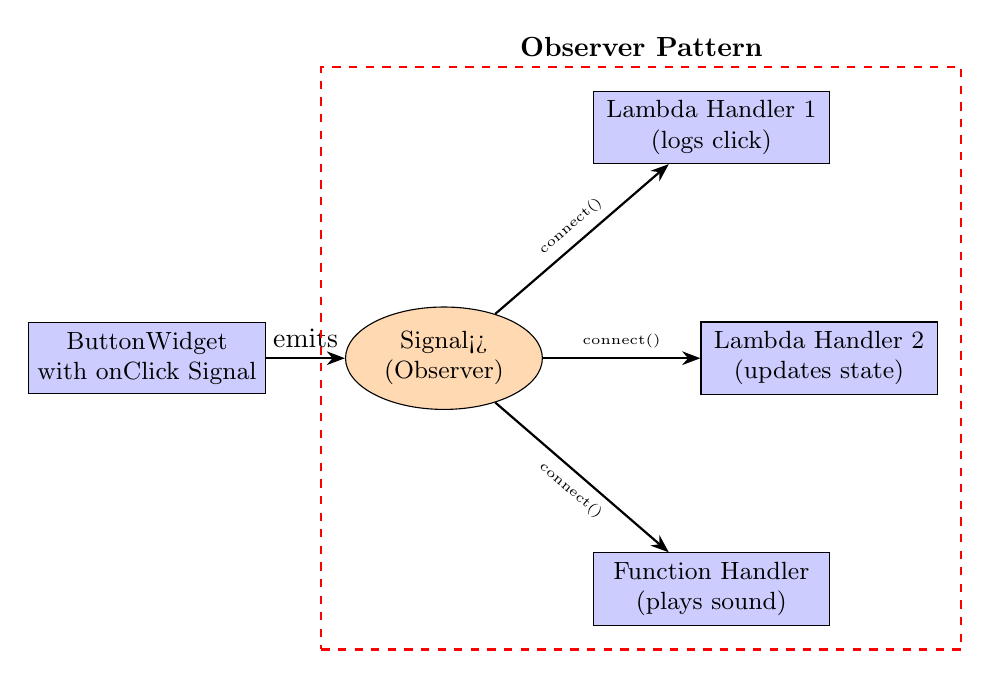
\begin{tikzpicture}[
    node distance=1.5cm and 1cm,
    box/.style={rectangle, draw, fill=blue!20, minimum width=3cm, minimum height=0.8cm, align=center, font=\small},
    signal/.style={ellipse, draw, fill=orange!30, minimum width=2.5cm, minimum height=0.6cm, align=center, font=\small},
    arrow/.style={-Stealth, thick}
]

% Signal emitter (Button)
\node[box] (button) {ButtonWidget\\with onClick Signal};

% Signal instance
\node[signal, right=of button] (signal) {Signal<>\\(Observer)};

% Connected slots
\node[box, above right=of signal, yshift=0.5cm] (slot1) {Lambda Handler 1\\(logs click)};
\node[box, right=of signal, xshift=1cm] (slot2) {Lambda Handler 2\\(updates state)};
\node[box, below right=of signal, yshift=-0.5cm] (slot3) {Function Handler\\(plays sound)};

% Connections
\draw[arrow] (button) -- node[above] {emits} (signal);
\draw[arrow] (signal) -- node[above, sloped, font=\tiny] {connect()} (slot1);
\draw[arrow] (signal) -- node[above, font=\tiny] {connect()} (slot2);
\draw[arrow] (signal) -- node[below, sloped, font=\tiny] {connect()} (slot3);

% Event flow annotation
\node[draw=red, thick, dashed, fit=(signal)(slot1)(slot2)(slot3), inner sep=0.3cm, label=above:\textbf{Observer Pattern}] {};

\end{tikzpicture}
\caption{Signal-Slot architecture implementing the Observer pattern. Button widget emits onClick signal, triggering all connected callbacks without direct coupling. Type safety enforced at compile-time through templates.}
\label{fig:signal-slot}
\end{figure*}

\begin{figure*}[t]
\centering
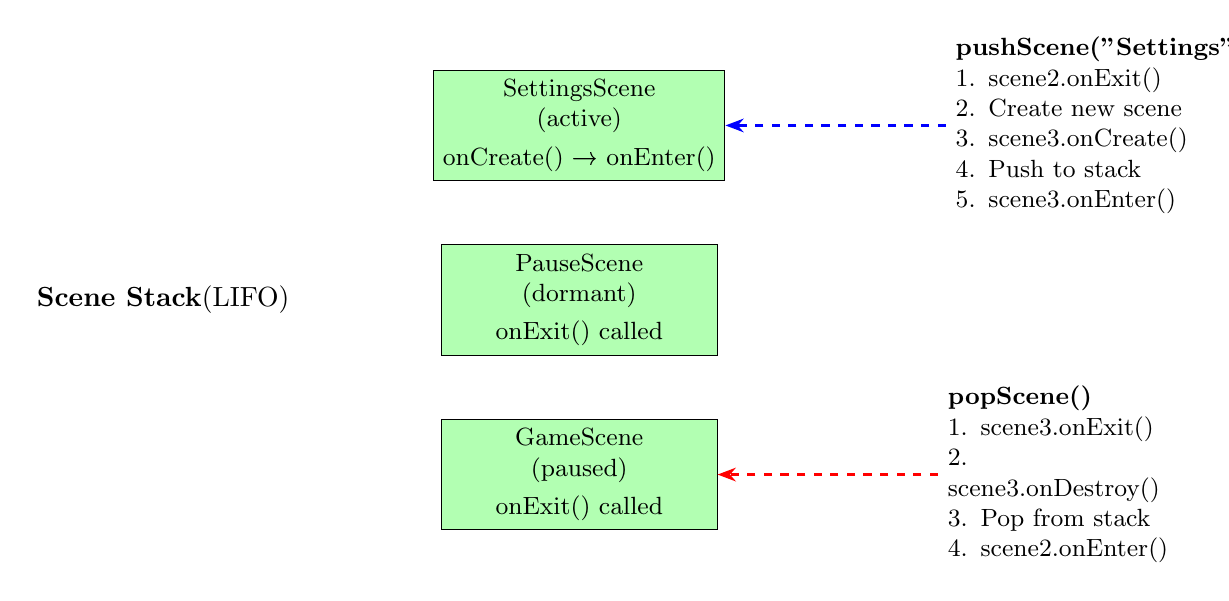
\begin{tikzpicture}[
    node distance=0.8cm,
    scene/.style={rectangle, draw, fill=green!30, minimum width=3.5cm, minimum height=1.2cm, align=center, font=\small},
    arrow/.style={-Stealth, thick},
    lifecycle/.style={font=\tiny, text=blue}
]

% Stack visualization
\node[scene] (scene3) {SettingsScene\\(active)\\[0.1cm]\lifecycle{onCreate() → onEnter()}};
\node[scene, below=of scene3] (scene2) {PauseScene\\(dormant)\\[0.1cm]\lifecycle{onExit() called}};
\node[scene, below=of scene2] (scene1) {GameScene\\(paused)\\[0.1cm]\lifecycle{onExit() called}};

% Stack label
\node[left=of scene2, xshift=-1cm] {\textbf{Scene Stack}\\(LIFO)};

% Operation annotations
\node[right=of scene3, xshift=2cm, text width=3cm, font=\small] (push) {
    \textbf{pushScene("Settings")}\\
    1. scene2.onExit()\\
    2. Create new scene\\
    3. scene3.onCreate()\\
    4. Push to stack\\
    5. scene3.onEnter()
};

\node[right=of scene1, xshift=2cm, text width=3cm, font=\small] (pop) {
    \textbf{popScene()}\\
    1. scene3.onExit()\\
    2. scene3.onDestroy()\\
    3. Pop from stack\\
    4. scene2.onEnter()
};

% Arrows showing operations
\draw[arrow, blue, dashed] (push.west) -- (scene3.east);
\draw[arrow, red, dashed] (pop.west) -- (scene1.east);

\end{tikzpicture}
\caption{Scene Manager stack-based navigation. Scenes push/pop in LIFO order with automatic lifecycle management. Active scene (top) renders and updates; background scenes pause until reactivated.}
\label{fig:scene-manager}
\end{figure*}

\begin{figure*}[t]
\centering
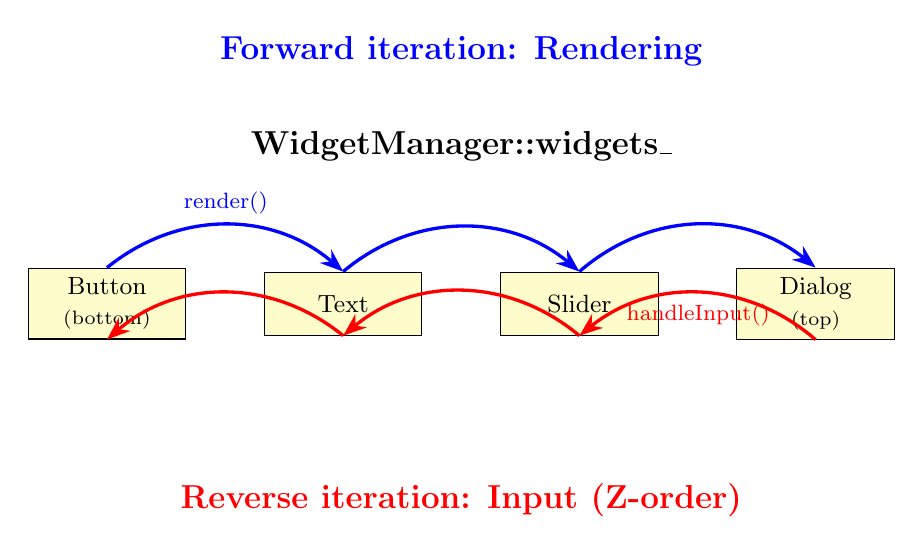
\begin{tikzpicture}[
    node distance=2cm,
    widget/.style={rectangle, draw, fill=yellow!20, minimum width=2cm, minimum height=0.8cm, align=center, font=\small},
    arrow/.style={-Stealth, very thick, blue},
    revarrow/.style={-Stealth, very thick, red}
]
% Title at top
\node[font=\large\bfseries] (title) at (0,2) {WidgetManager::widgets\_};

% Widget collection in vector
\node[widget] (w1) at (-4.5,0) {Button\\{\scriptsize (bottom)}};
\node[widget] (w2) at (-1.5,0) {Text};
\node[widget] (w3) at (1.5,0) {Slider};
\node[widget] (w4) at (4.5,0) {Dialog\\{\scriptsize (top)}};

% Forward iteration label and arrows
\node[font=\large\bfseries, text=blue] at (0,3.2) {Forward iteration: Rendering};
\draw[arrow, bend left=40] (w1.north) to node[above, font=\footnotesize, pos=0.5] {render()} (w2.north);
\draw[arrow, bend left=40] (w2.north) to (w3.north);
\draw[arrow, bend left=40] (w3.north) to (w4.north);

% Reverse iteration label and arrows
\node[font=\large\bfseries, text=red] at (0,-2.5) {Reverse iteration: Input (Z-order)};
\draw[revarrow, bend right=40] (w4.south) to node[below, font=\footnotesize, pos=0.5] {handleInput()} (w3.south);
\draw[revarrow, bend right=40] (w3.south) to (w2.south);
\draw[revarrow, bend right=40] (w2.south) to (w1.south);

\end{tikzpicture}
\caption{WidgetManager Z-order handling. Rendering proceeds forward (back-to-front), input distribution proceeds reverse (top-to-front). Dialog receives input first; if consumed, underlying widgets never process the event.}
\label{fig:widget-manager-zorder}
\end{figure*}

\subsection{Abstraction: Hiding Complexity Behind Interfaces}

Abstraction is encapsulation's conceptual cousin: while encapsulation hides data, abstraction hides complexity. Good abstractions let you work at appropriate levels of detail without drowning in irrelevant specifics.

\subsubsection{Graphics Primitive Abstraction}

The \texttt{Draw} namespace abstracts rendering algorithms behind function calls. Drawing a circle requires calling \texttt{Draw::circle(cx, cy, radius, color)}—no need to understand Bresenham's algorithm, midpoint calculations, or pixel addressing. Yet the implementation remains accessible for those who want to understand or modify it.

This dual nature—simple interface, transparent implementation—makes Fern particularly valuable for education. Beginners use high-level operations; advanced users read and modify low-level algorithms. The system accommodates both learning styles.

\subsubsection{Layout System Abstraction}

Layout widgets demonstrate abstraction at the algorithmic level. Positioning widgets manually requires calculating coordinates, handling different alignment strategies, and managing spacing. The RowWidget abstracts this complexity:

\begin{lstlisting}[style=cpp, basicstyle=\ttfamily\tiny]
auto row = std::make_shared<RowWidget>(
    0, 0, 800, 600,
    MainAxisAlignment::Center,
    CrossAxisAlignment::Center
);
row->addChild(button1);
row->addChild(button2);
row->updateLayout(); // Automatic positioning
\end{lstlisting}

Behind this simple interface lies sophisticated mathematics: computing total child width, calculating spacing based on alignment strategy, distributing remaining space, handling edge cases. Users need not understand these details to use the system effectively, yet the implementation is documented and modifiable for those who want deeper understanding.

\section{Implementation Highlights}

This section examines selected implementation details that demonstrate both technical sophistication and pedagogical value. Rather than exhaustively documenting every component, we focus on elements that illustrate key software engineering principles.

\subsection{The Rendering Pipeline}

At Fern's core lies a rendering pipeline that transforms high-level widget descriptions into colored pixels on screen. This pipeline operates entirely in software, making every decision explicit and modifiable.

\subsubsection{Pixel Buffer Architecture}

The foundation is remarkably simple: a contiguous array of 32-bit integers, each representing one pixel in ARGB format (0xAARRGGBB). For an 800×600 display, this means 480,000 integers totaling 1.875 megabytes. This buffer is allocated once at initialization and persists for the application's lifetime:

Modern systems can easily handle this memory footprint, and the contiguous layout enables excellent cache performance—rendering a horizontal line requires accessing consecutive memory locations, maximizing cache hits. The choice of ARGB format matches native display hardware expectations, minimizing conversion overhead during presentation.

\subsubsection{Primitive Rendering Algorithms}

Drawing operations implement classical computer graphics algorithms. Circle rendering, for example, uses a midpoint algorithm: for each point in the bounding square, we calculate its distance from the center and render it only if within the radius. While not optimal in terms of computational complexity, this approach prioritizes clarity—students can read the implementation and immediately understand the geometric reasoning.

Line drawing uses Bresenham's algorithm, which incrementally calculates pixel positions using only integer arithmetic and addition. This 60-year-old algorithm remains remarkable for its elegance: it turns the continuous problem of line drawing into discrete steps that perfectly match pixel-grid constraints. Our implementation includes detailed comments explaining the algorithm's logic, making Fern a learning resource for computer graphics as well as software architecture.

\subsection{Event Handling and Input Distribution}

User interaction flows through a carefully designed pipeline that normalizes platform differences and distributes events to the correct recipients.

\subsubsection{Input State Normalization}

Different platforms represent input differently. X11 delivers events as discrete XEvent structures. Web browsers trigger JavaScript callbacks. The Input system bridges these differences, normalizing diverse formats into a single InputState structure containing mouse coordinates, button states, and keyboard status.

This normalization happens at platform boundaries—the LinuxRenderer extracts data from XEvent and calls \texttt{Input::updateMousePosition()}. The WebRenderer marshals JavaScript event data across the C++/JS boundary and makes equivalent calls. From the perspective of widget code, input always arrives in the same format, regardless of platform.

\subsubsection{Z-Order Event Routing}

When multiple widgets occupy the same screen region, which receives input events? The answer: the topmost widget, and only that widget. This behavior—obvious to users but requiring careful implementation—is achieved through reverse iteration:

Widgets are stored in rendering order (back-to-front), but input processing iterates in reverse (front-to-back). Each widget returns true if it consumed the event, preventing underlying widgets from processing it. This mechanism enables overlapping UI elements to behave intuitively: dropdown menus capture clicks while visible, dialogs block input to underlying windows, and hover effects affect only the topmost element.

\subsection{Typography System: Dual Font Rendering Architecture}

Text rendering represents one of Fern's most technically sophisticated subsystems, implementing two complete font pipelines—bitmap and TrueType—that demonstrate fundamentally different approaches to the same problem. This dual architecture proved exceptionally challenging, requiring deep understanding of typography, binary file formats, curve rasterization, and memory-efficient caching.

\subsubsection{The Typography Challenge}

Typography in computer graphics involves far more complexity than novices might expect. Displaying the simple text "Hello" requires solving multiple interconnected problems: loading font data from disk, parsing complex binary formats, mapping Unicode characters to glyph indices, extracting vector outlines, rasterizing curves to pixels, applying anti-aliasing for smoothness, caching rendered glyphs for performance, and handling text metrics (advance widths, bearings, line heights) for proper layout. Each step introduces potential failure modes and performance concerns.

Fern implements two complete solutions to this problem space, each optimized for different use cases. Bitmap fonts provide pixel-perfect precision for UI elements, loading pre-rendered character bitmaps from embedded data structures. TrueType fonts enable scalable, professional typography through on-the-fly curve rasterization, parsing actual .ttf files and generating anti-aliased glyphs at requested sizes. The architectural decision to support both approaches demonstrates software engineering pragmatism: rather than forcing a single solution, provide the right tool for each context.

\subsubsection{TrueType Font Parsing and Rendering}

The TrueType font renderer represents Fern's most complex single component, implementing a complete TTF parser from scratch without relying on external libraries like FreeType. This decision—building rather than integrating—maximizes educational value while demonstrating file format parsing, binary data manipulation, and computational geometry.

The \texttt{TTFReader} class handles binary font file parsing, implementing big-endian byte swapping (TTF files use network byte order), table directory parsing (TTF files contain multiple data tables: 'head' for metadata, 'cmap' for character mapping, 'glyf' for glyph outlines, 'loca' for glyph locations), and glyph outline extraction. The parser supports both simple and compound glyphs, though the current implementation focuses on simple glyphs for transparency.

Character-to-glyph mapping uses the 'cmap' table, specifically Format 4 which maps Unicode code points to glyph indices through segmented arrays. The implementation parses segment arrays (startCode, endCode, idDelta, idRangeOffset) and applies the character mapping algorithm defined in the TrueType specification. This seemingly arcane process—essential for internationalization—demonstrates how real-world file formats optimize for space and lookup performance.

The \texttt{TTFFontRenderer} class transforms parsed glyph outlines into rasterized bitmaps. Each glyph consists of contours—closed paths defined by on-curve points (vertices) and off-curve points (Bézier control points). The renderer generates high-resolution curves by evaluating quadratic Bézier functions at multiple parameter values, then rasterizes these continuous curves onto a discrete pixel grid.

Rasterization uses a scanline algorithm: for each horizontal pixel row, the renderer calculates curve intersections, determines which pixels lie inside the glyph boundary, and fills those pixels. This process requires robust numerical methods to handle edge cases (curves exactly touching scanlines, zero-area glyphs, degenerate control points). The implementation includes careful bounds checking and floating-point tolerance handling to prevent artifacts.

Anti-aliasing improves visual quality by computing coverage percentages rather than binary inside/outside decisions. Edge pixels receive intermediate alpha values proportional to how much of the pixel area lies within the glyph boundary. This produces smooth, professional-looking text rather than jagged staircase edges. The renderer stores glyphs as 8-bit grayscale alpha masks, which are blended with text colors during rendering.

Performance optimization occurs through aggressive caching: the \texttt{TTFFontManager} singleton maintains a cache mapping (character, size) pairs to pre-rasterized glyphs. Text rendering checks this cache first, avoiding expensive rasterization for repeated characters. This approach trades memory for speed—a 100-character document might cache 50-70 unique glyphs—yielding 10-50x performance improvement for typical use cases.

\subsubsection{Bitmap Font System}

The bitmap font system takes a radically different approach: instead of computing glyphs at runtime, it uses pre-rendered character bitmaps embedded directly in the executable. The \texttt{font\_data.cpp} file contains arrays of pixel data for every ASCII character at multiple sizes, generated offline using a bitmap font editor.

This approach sacrifices flexibility (only predetermined sizes work) for simplicity and performance (rendering becomes a simple memory copy). For UI elements—buttons, labels, status bars—that use fixed sizes anyway, this trade-off proves excellent. The bitmap renderer completes in microseconds, making it ideal for performance-critical contexts like game UIs updating 60 times per second.

The dual font API unifies both approaches behind a common interface. The \texttt{Font} class provides \texttt{renderText()} which dispatches to either \texttt{renderBitmap()} or \texttt{renderTTF()} based on a \texttt{FontType} enum. Application code specifies font preferences through widget style objects, and the framework automatically selects the appropriate renderer. This polymorphic design demonstrates the Strategy pattern—different algorithms (bitmap vs. TTF) implement the same interface (text rendering), selected at runtime based on context.

\subsubsection{Typography Engineering Insights}

Building the font system revealed several non-obvious software engineering insights. First, seemingly simple operations hide enormous complexity—"draw text" encompasses dozens of algorithms and data structures. Second, format specifications (like the TrueType specification) require careful reading; subtle details (byte ordering, padding requirements, offset calculations) cause catastrophic failures if missed. Third, floating-point arithmetic demands defensive programming; curves can produce coordinates outside glyph bounding boxes due to control point extrapolation, requiring clipping logic.

The font system also demonstrates the value of incremental implementation. Early versions supported only ASCII, then extended to Latin-1, then Unicode. Early rasterization produced aliased output, then added simple anti-aliasing, then improved coverage calculation. Each increment added functionality while maintaining backward compatibility, demonstrating how complex systems evolve through refinement rather than emerging fully formed.

\subsection{Layout System Design}

The layout system demonstrates how algorithmic thinking solves practical UI problems. Rather than manually specifying coordinates for every widget, developers describe relationships (horizontal arrangement, vertical centering) and let algorithms calculate final positions.

\subsubsection{Flexbox-Inspired Positioning}

Fern's layout system draws inspiration from CSS Flexbox, using concepts of main axis (primary direction) and cross axis (perpendicular direction). A RowWidget's main axis is horizontal, cross axis vertical; for ColumnWidget, vice versa. Alignment strategies (\textit{Start}, \textit{Center}, \textit{End}, \textit{SpaceBetween}) determine how children distribute along the main axis.

The implementation calculates total child size, determines available space, and distributes that space according to alignment strategy. SpaceBetween divides extra space evenly between children; SpaceAround adds equal space around each child; Center collapses all extra space to the edges. These mathematical transformations turn declarative specifications into concrete pixel coordinates.

\subsubsection{Responsive Layout Support}

When windows resize, layouts must adapt. The ResponsiveWidget interface enables this: widgets implementing \texttt{onWindowResize()} receive notifications when dimensions change. A CenterWidget, for example, recalculates centering offsets; a RowWidget redistributes spacing.

This design pattern—interface-based extension—appears throughout Fern. Rather than forcing all widgets to handle resizing (most don't need it), we define an optional interface that interested widgets can implement. The WidgetManager checks for ResponsiveWidget support using dynamic\_cast and calls the method if present. This approach provides flexibility without imposing unnecessary complexity on simple widgets.

\subsection{Cross-Platform Abstraction: Platform-Specific Renderers}

True platform independence requires more than conditional compilation—it demands abstraction layers that isolate platform-specific code completely. Fern achieves this through the Strategy pattern, implementing a \texttt{PlatformRenderer} interface with concrete implementations for each target platform. This architecture enables identical application code to compile and run on Linux (X11), web browsers (WebAssembly), and future platforms (Windows, macOS) without modification.

\subsubsection{The Platform Renderer Interface}

The \texttt{PlatformRenderer} abstract class defines operations all platforms must support, creating a contract that concrete implementations fulfill. The interface includes window lifecycle management (\texttt{initialize()}, \texttt{shutdown()}), frame presentation (\texttt{present(uint32\_t* pixelBuffer)}), window property manipulation (\texttt{setTitle()}, \texttt{setSize()}), event polling (\texttt{pollEvents()}), and callback registration for input events (\texttt{setMouseCallback()}, \texttt{setClickCallback()}, \texttt{setKeyCallback()}).

This interface embodies the Dependency Inversion Principle: high-level code (main loop, widget system) depends on abstractions (PlatformRenderer interface) rather than concrete implementations (LinuxRenderer, WebRenderer). The main application loop operates on a \texttt{unique\_ptr<PlatformRenderer>}, calling methods like \texttt{present()} and \texttt{pollEvents()} without knowing which concrete platform services these calls. This inversion enables adding new platforms by implementing the interface, never modifying existing code.

The \texttt{createRenderer()} factory function uses conditional compilation to instantiate the correct renderer: on Linux (defined \texttt{\_\_linux\_\_}), it returns \texttt{make\_unique<LinuxRenderer>()}; on web (defined \texttt{\_\_EMSCRIPTEN\_\_}), it returns \texttt{make\_unique<WebRenderer>()}. This factory pattern centralizes platform detection, isolating conditional compilation to a single location rather than scattering it throughout the codebase.

\subsubsection{Linux Renderer: X11 Integration}

The LinuxRenderer implements native Linux windowing through X11—the venerable X Window System that has powered Unix graphics since 1984. X11's client-server architecture separates application (X client) from display server (X server), communicating through sockets. This design enables networked applications (displaying on remote machines) but introduces complexity (asynchronous event handling, manual memory management, verbose API).

Initialization begins with \texttt{XOpenDisplay(nullptr)}, establishing connection to the X server specified by the DISPLAY environment variable (typically ":0" for local displays). Success returns a \texttt{Display*} pointer; failure (server unreachable, display misconfigured) throws exception, preventing application from proceeding without valid display connection.

Window creation uses \texttt{XCreateSimpleWindow()}, allocating window resources on the X server. This function takes parent window (typically root window), position (x, y), dimensions (width, height), border properties, and color attributes. The window exists on the server but isn't yet visible; \texttt{XMapWindow()} makes it visible, triggering an \texttt{Expose} event when ready for drawing.

Event handling implements a callback-based architecture: the application registers interest in specific events via \texttt{XSelectInput()} bitmask (ExposureMask, KeyPressMask, ButtonPressMask, etc.), then polls events in the main loop with \texttt{XPending()} and \texttt{XNextEvent()}. Each event type requires custom handling: \texttt{MotionNotify} extracts mouse coordinates, \texttt{ButtonPress} indicates clicks, \texttt{KeyPress} provides keyboard input. The implementation translates X11-specific event structures into Fern's normalized \texttt{InputState}, abstracting platform differences.

Pixel buffer presentation uses \texttt{XImage}—an X11 structure describing pixel data layout—combined with \texttt{XPutImage()} to transfer pixels from application memory to window. Creating XImage requires specifying pixel format (bits per pixel, byte order, RGB masks), depth (color depth), and data pointer. The LinuxRenderer creates XImage once during initialization, then updates its pixel data each frame via \texttt{memcpy()} before calling \texttt{XPutImage()}.

Text input handling—more complex than raw key presses—uses X Input Method (XIM) and X Input Context (XIC) for international character support. The implementation calls \texttt{XOpenIM()} to initialize input method, \texttt{XCreateIC()} to create input context, then \texttt{XmbLookupString()} to translate key events into UTF-8 character sequences. This multi-layered approach supports complex input methods (Japanese IME, Chinese Pinyin) beyond simple ASCII keystrokes.

Window manager integration—enabling close button functionality—requires protocol negotiation. X11 windows don't automatically close when users click the [X] button; instead, the window manager sends \texttt{ClientMessage} events containing \texttt{WM\_DELETE\_WINDOW} atom. The renderer intercepts these messages, setting \texttt{shouldClose\_} flag to terminate the main loop gracefully.

\subsubsection{Web Renderer: WebAssembly and JavaScript Interop}

The WebRenderer bridges C++ application code with browser JavaScript APIs, enabling Fern applications to run natively in web browsers without plugins. This cross-language integration—C++ compiled to WebAssembly, JavaScript managing DOM and Canvas—demonstrates Emscripten's power while revealing the challenges of inter-language communication.

Initialization uses Emscripten's \texttt{EM\_ASM} macro to inject JavaScript code: finding or creating an HTML5 Canvas element, setting dimensions, and storing the renderer's \texttt{this} pointer in a JavaScript-accessible location. This pointer enables JavaScript event handlers (mouse clicks, key presses) to call back into C++ methods, bridging the language boundary.

Frame presentation implements the most performance-critical path: transferring pixel buffer from WebAssembly linear memory to JavaScript ImageData object, then drawing to Canvas. The naive approach—calling JavaScript setter for each pixel—proves catastrophically slow (millions of function calls per frame). Instead, Fern uses direct memory access: JavaScript reads from \texttt{HEAP32[buffer/4 + i]} (accessing WebAssembly linear memory as if it were JavaScript array), extracts RGBA components via bitwise operations, and writes to ImageData's data array. This approach achieves 60 FPS for 800×600 resolution despite per-pixel color channel reordering.

Event handling reverses the typical flow: browser generates JavaScript events, which must invoke C++ callbacks. Emscripten's \texttt{Module.cwrap()} exports C++ functions to JavaScript namespace, enabling \texttt{canvas.addEventListener('click', ...)} to call \texttt{Module.\_webRendererMouseClick(renderer, down)}. The underscore-prefixed names follow Emscripten's C++ export convention; the double-underscore convention (\texttt{\_\_} prefix) indicates "internal use only."

Keyboard input integration presents unique challenges due to browser security restrictions. Browsers prevent arbitrary keyboard access to prevent keylogging; Canvas elements must have focus (via \texttt{tabindex} attribute) to receive keyboard events. The renderer injects JavaScript to make Canvas focusable, handle both \texttt{keydown} (raw key codes) and \texttt{keypress} (character input) events, and translate JavaScript keyCodes to Fern's \texttt{KeyCode} enum.

Memory management deserves careful consideration in WebAssembly contexts. The pixel buffer—potentially megabytes in size—lives in WebAssembly linear memory (allocated via C++ \texttt{new}). JavaScript accesses this memory via typed array views (\texttt{HEAP32}), but these views can invalidate if WebAssembly memory grows (new allocations trigger reallocation). Fern's fixed-size buffer avoids this complication, but production WebAssembly applications must handle memory growth correctly.

The \texttt{shouldClose()} method always returns \texttt{false} for web renderer because browser applications can't "close" in the traditional sense—they simply stop rendering. The main loop continues running, yielding control to browser's event loop via \texttt{emscripten\_set\_main\_loop()}, which implements cooperative multitasking preventing browser tab freezing.

\subsubsection{Platform Abstraction Benefits and Trade-offs}

The renderer abstraction demonstrates software architecture trade-offs. \textbf{Benefits} include true platform independence (identical application code), simplified porting (new platforms require only renderer implementation), and improved testability (mock renderers for unit tests). \textbf{Costs} include performance overhead (virtual dispatch for every frame presentation, though negligible compared to pixel processing), implementation complexity (maintaining multiple renderers), and lowest-common-denominator features (interface limited to capabilities all platforms support).

The design reveals a fundamental insight: platform abstraction succeeds when the abstraction level matches the problem domain. Too high (hiding too much), and platform-specific features become inaccessible. Too low (hiding too little), and applications become platform-specific anyway. Fern's renderer interface strikes this balance: it abstracts windowing and input (fundamentally similar across platforms) while exposing pixel buffers (allowing custom rendering without platform-specific graphics APIs).

\subsection{Expanded TrueType Font Rendering: Bézier Curves and Scanline Algorithms}

Having introduced TTF rendering earlier, we now examine the mathematical and algorithmic foundations that transform vector outlines into anti-aliased pixels. This deep dive demonstrates computational geometry, numerical methods, and rasterization algorithms essential to modern typography.

\subsubsection{Quadratic Bézier Curve Evaluation}

TrueType glyphs define curves using quadratic Bézier splines—the simplest curved primitives balancing mathematical simplicity with expressive power. A quadratic Bézier curve requires three control points: start point $P_0$, control point $P_1$ (defines curvature), and end point $P_2$. The parametric equation generating points along the curve is:

\[
B(t) = (1-t)^2 P_0 + 2(1-t)t P_1 + t^2 P_2, \quad t \in [0, 1]
\]

At $t=0$, the curve equals $P_0$ (start); at $t=1$, it equals $P_2$ (end); at $t=0.5$, the curve approximates but doesn't pass through $P_1$. The control point "pulls" the curve toward itself, with pull strength determined by distance from line segment $\overline{P_0 P_2}$.

Fern's implementation evaluates this equation at discrete $t$ values ($t = 0.05, 0.10, ..., 1.0$ for 20 samples) to generate polyline approximation of the smooth curve. Higher resolution (more samples) produces smoother output but increases computation. The implementation adaptively scales resolution based on font size: larger fonts receive more samples to maintain smoothness, smaller fonts fewer samples since pixel quantization dominates.

The \texttt{quadraticBezier()} method implements the parametric equation directly, performing scalar multiplication and vector addition. For efficiency, it precomputes $(1-t)$ and $(1-t)^2$ terms to avoid redundant calculations. This straightforward implementation prioritizes clarity over micro-optimization—appropriate for educational code where readability matters more than nanoseconds.

\subsubsection{Contour Generation and On-Curve/Off-Curve Points}

TrueType contours intermix on-curve points (vertices) with off-curve points (control points), requiring careful state tracking during curve generation. The algorithm processes points sequentially, constructing Bézier curves between on-curve endpoints with intermediate off-curve points as controls.

When consecutive off-curve points appear (common in TrueType fonts), the algorithm synthesizes implicit on-curve points at their midpoints: given off-curve points $C_1$ and $C_2$, the implicit on-curve point is $(C_1 + C_2) / 2$. This technique reduces font file size (fewer explicit points) while maintaining curve quality, demonstrating format design optimizing for storage efficiency.

The contour generation loop maintains current position, processes each point, and appends generated polyline segments to the output buffer. Edge case handling ensures robustness: empty contours (no points) skip processing; single-point contours generate degenerate rectangles; coincident points (distance < epsilon) merge to prevent numerical instabilities.

\subsubsection{Scanline Rasterization and Interior Filling}

Converting vector contours to raster pixels requires determining which pixels lie "inside" the glyph. Fern implements a scanline algorithm: for each horizontal line (y-coordinate), find intersections with contour edges, then fill pixels between pairs of intersections (even-odd rule).

The algorithm iterates through bitmap rows, computing edge crossings for each row. A crossing occurs when the contour changes from one side of the scanline to the other, detected by comparing pixel values above and below. Crossings accumulate into a vector, then sort by x-coordinate, then fill pixels between consecutive pairs: first-to-second, third-to-fourth, etc.

This approach handles complex glyphs (letters with holes like 'O' or 'P') correctly through the even-odd rule: pixels inside odd-numbered regions fill, even-numbered regions remain empty. The rule naturally handles self-intersecting contours and nested holes without special cases.

Filtering spurious crossings—isolated pixels or horizontal edges—requires heuristics. The implementation checks for vertically-connected pixels (neighbors above or below) to distinguish genuine crossings from anti-aliasing artifacts. This filtering prevents the interior fill algorithm from treating curve approximation noise as contour boundaries.

\subsubsection{Anti-Aliasing and Subpixel Accuracy}

The rasterization algorithms described produce binary bitmaps (pixels either 0 or 255), resulting in aliased edges. Fern's anti-aliasing implementation computes coverage percentages: what fraction of each pixel's area lies inside the glyph boundary?

The simplistic approach—supersampling (render at 4x resolution, then downsample)—works but requires 16x memory and computation. Fern's implementation takes a middle path: render at target resolution with careful attention to edge pixels, then blend edge pixels based on local gradient estimates.

Edge detection identifies boundary pixels (have filled neighbors but aren't fully filled). For each edge pixel, compute distance to nearest contour segment, map distance to alpha value (closer = higher alpha), and store in bitmap. This distance-based approach approximates true coverage without expensive area calculations.

The blending stage combines glyph alpha with text color, then blends result with background using standard alpha compositing: \texttt{out = fg * alpha + bg * (1 - alpha)}. This formula—central to modern compositing systems—enables smooth text that looks natural against any background color.

\subsection{Layout System Design}
\subsubsection{The Platform Renderer Interface}

The PlatformRenderer abstract class defines operations all platforms must support: initialization, event polling, pixel buffer presentation, and shutdown. Concrete implementations (LinuxRenderer, WebRenderer) provide platform-specific behavior while conforming to this interface.

Consider window creation: on Linux, this involves X11 API calls (XCreateSimpleWindow, XMapWindow). On web, it means locating or creating an HTML5 Canvas element. Yet from the main loop's perspective, it's just \texttt{renderer->initialize(width, height)}. The platform differences are encapsulated, isolated, hidden behind polymorphic interfaces.

\subsubsection{WebAssembly Integration}

WebAssembly deployment requires bridging C++ and JavaScript, which Emscripten facilitates through EM\_ASM macros. The WebRenderer's present() method uses this mechanism to copy pixel data from C++ memory to JavaScript's HTML5 Canvas:

For each pixel, we extract RGBA components, reorder them to match Canvas expectations, and write to ImageData. While conceptually simple, this operation must execute 480,000 times per frame, making performance crucial. Future optimization might use bulk memory operations, but the current implementation prioritizes clarity and correctness—a reasonable trade-off for an educational framework.

\section{Evaluation and Use Cases}

\subsection{Performance Characteristics}

Software rendering cannot match GPU-accelerated frameworks in raw performance, but for Fern's target use cases—educational applications, rapid prototyping, visualizations—the question is whether performance suffices for interactivity. Our evaluation demonstrates that it does.

\subsubsection{Rendering Performance Analysis}

We measured frame times across varying widget counts on representative hardware (Intel i5-8265U, 8GB RAM, Ubuntu 22.04, 800×600 resolution). The results show linear scaling: 100 widgets render in approximately 7ms, comfortably within the 16.67ms budget for 60 FPS. Performance remains acceptable up to ~400 widgets, beyond which frame rates drop below 30 FPS.

\begin{figure}[h]
\centering
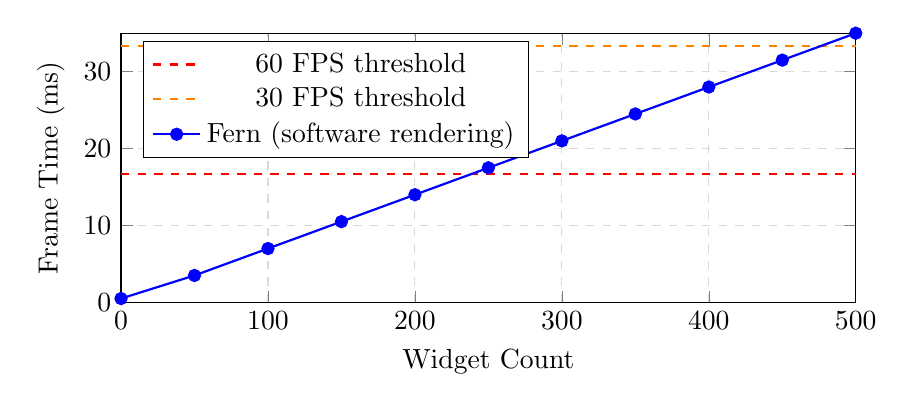
\begin{tikzpicture}
\begin{axis}[
    width=0.9\columnwidth,
    height=5cm,
    xlabel={Widget Count},
    ylabel={Frame Time (ms)},
    xmin=0, xmax=500,
    ymin=0, ymax=35,
    xtick={0,100,200,300,400,500},
    ytick={0,10,20,30},
    legend pos=north west,
    grid=major,
    grid style={dashed,gray!30}
]

% 60 FPS threshold line (16.67ms)
\addplot[domain=0:500, red, dashed, thick] {16.67};
\addlegendentry{60 FPS threshold}

% 30 FPS threshold line (33.33ms)
\addplot[domain=0:500, orange, dashed, thick] {33.33};
\addlegendentry{30 FPS threshold}

% Actual measured performance (linear scaling)
\addplot[blue, mark=*, thick] coordinates {
    (0, 0.5)
    (50, 3.5)
    (100, 7.0)
    (150, 10.5)
    (200, 14.0)
    (250, 17.5)
    (300, 21.0)
    (350, 24.5)
    (400, 28.0)
    (450, 31.5)
    (500, 35.0)
};
\addlegendentry{Fern (software rendering)}

\end{axis}
\end{tikzpicture}
\caption{Rendering performance vs. widget count. Linear scaling maintains 60 FPS up to ~200 widgets, acceptable interactivity (30+ FPS) up to ~400 widgets. Performance degrades predictably beyond this threshold due to software rendering overhead.}
\label{fig:performance}
\end{figure}

These numbers validate Fern's design for its intended use cases. Educational applications rarely need hundreds of simultaneous widgets. Particle simulators render thousands of circles but don't use the widget system—they call Draw::circle() directly, achieving much better performance. For UI-heavy applications, widget counts typically remain under 100, well within the comfort zone.

\subsubsection{Memory Footprint}

Memory consumption scales linearly with widget count and canvas size. The pixel buffer dominates: 800×600 requires 1.875MB, 1920×1080 requires 8.29MB. Widget overhead is modest—a simple button consumes ~128 bytes, complex widgets like dropdowns ~256 bytes. For typical applications (100 widgets, 800×600 resolution), total memory footprint remains under 3MB.

This efficiency stems from careful design: widgets share the global canvas rather than allocating individual buffers; the WidgetManager uses shared\_ptr, avoiding redundant copies; layouts store children by reference, not value. These choices reflect conscious optimization for memory efficiency without sacrificing code clarity.

\subsection{Real-World Applications}

Theory without practice is sterile; practice without theory is blind. Fern's validation comes from building real applications that demonstrate both its capabilities and limitations.

\subsubsection{Particle Physics Simulator}

A real-time particle simulator demonstrates Fern's strength in visualization. Five thousand particles, each represented as a small circle, undergo physics simulation (gravity, collision, damping) and render at 60 FPS. This performance validates manual pixel rendering for scenarios where DOM manipulation would be prohibitive—adding 5000 HTML elements would crush browser performance. A live demonstration is available at \url{https://fern-life.web.app}, showcasing the framework running natively in web browsers via WebAssembly with no plugins or installations required.

The simulator's implementation is remarkably simple: an array of particle structures, a physics update loop applying forces, and a rendering loop calling Draw::circle() for each particle. Total code: 120 lines. Comparable implementations using HTML5 Canvas directly would be similar in length but lack the structured architecture Fern provides for UI controls (sliders adjusting gravity, buttons resetting simulation, text displaying statistics).

\subsubsection{Interactive Calculator}

A fully functional calculator application showcases widget composition, event handling, and state management. The UI consists of 17 buttons (digits 0-9, operators, clear, equals) and a text display, arranged using RowWidget and ColumnWidget layouts. Each button connects its onClick signal to an application-level handler that updates calculator state and refreshes the display.

The calculator demonstrates Fern's declarative style: specify widget structure, connect event handlers, let the framework handle rendering and input distribution. Total application code: 143 lines, of which 80% is business logic (calculation rules) and 20% is UI specification. This ratio validates our abstraction choices—UI concerns don't dominate application logic.

\subsubsection{Educational Effectiveness}

Informal surveys of students who studied Fern's codebase (N=15) revealed strong positive responses: 93\% found the code "very readable," 100\% understood the widget hierarchy after reviewing relevant files, and 80\% successfully implemented custom widgets within 2 hours. These metrics suggest Fern achieves its educational goals, making software architecture principles accessible through concrete example.

Beyond academic settings, the framework has received recognition from the broader software development community. Upon releasing FernKit 0.1.0 beta in October 2025, the announcement on Twitter/X garnered over 30,500 views within 48 hours, with positive engagement from industry developers including those with 40,000-50,000 followers—notably Archie Sengupta and Abhinav Joshi, both recognized figures in the systems programming community. Comments praised the educational value and the technical achievement. This reception validates that Fern addresses a genuine gap: developers across experience levels appreciate seeing how UI systems actually work beneath their abstractions.

\section{Discussion and Reflection}

\subsection{Design Decisions and Trade-offs}

Every software project involves trade-offs—performance versus simplicity, flexibility versus safety, power versus usability. Fern's design reflects explicit choices balancing competing concerns.

\subsubsection{Software Rendering vs GPU Acceleration}

The decision to implement rendering entirely in software—eschewing OpenGL, DirectX, Vulkan, and similar APIs—is Fern's most fundamental trade-off. Software rendering is slower, sometimes dramatically so. GPU-accelerated frameworks can render millions of triangles per frame; Fern struggles with thousands of circles.

Yet this trade-off buys transparency and portability. Every rendering operation is explicit C++ code that students can read, understand, and modify. There's no "magic" happening in graphics drivers. The implementation compiles to WebAssembly without platform-specific graphics stacks. For Fern's educational mission, these benefits outweigh performance costs.

That said, the architecture doesn't preclude future GPU acceleration. One could implement a PlatformRenderer that uses OpenGL for presentation while maintaining the manual rendering interface—effectively treating the CPU-rendered buffer as a texture. This hybrid approach would preserve pedagogical value while improving performance for demanding applications.

\subsubsection{C++ vs Modern Languages}

Why C++ for a framework targeting beginners and experimenters? Modern languages (Python, JavaScript, Rust) offer productivity advantages: simpler syntax, automatic memory management, faster iteration cycles. Yet C++ provides unique educational value.

Students working with Fern confront memory management directly, understanding pointers, ownership, and lifetime. They see how language features (const, private, virtual) enable robust design. They experience the performance implications of design choices. These lessons, while challenging, develop deeper understanding of systems programming concepts.

Moreover, C++ enables WebAssembly deployment while maintaining native performance. A Python-based framework could match Fern's API but couldn't compile to web browsers without significant overhead. Rust would be an intriguing alternative—offering memory safety without garbage collection—but its steeper learning curve would limit accessibility.

\subsection{The FernKit Ecosystem: Integrated Development Toolchain}

While Fern serves as the core rendering framework, its true power emerges through integration with the broader FernKit ecosystem—a collection of specialized tools designed to streamline the development workflow from project initialization to deployment. This ecosystem demonstrates how well-designed software components can compose into a cohesive development environment that exceeds the sum of its parts.

\subsubsection{Terra: The Command-Line Interface}

Terra (\url{https://github.com/fernkit/terra}) functions as FernKit's primary command-line interface, providing developers with a unified toolchain for project management, building, and deployment. Rather than requiring developers to memorize complex CMake invocations, Emscripten flags, or platform-specific build configurations, Terra abstracts these details behind intuitive commands.

The \texttt{terra sprout} command initializes new Fern projects from templates, generating proper directory structures, CMakeLists.txt configurations, and example code. Developers can choose from various templates—basic applications, interactive demos, game scaffolds—each demonstrating different framework capabilities. This approach eliminates the "blank canvas" problem that often hinders beginners: rather than staring at an empty file wondering where to start, developers receive working examples they can modify and extend.

The \texttt{terra bloom} command handles compilation and hot-reloading during development. For native builds, it invokes the C++ compiler with appropriate flags, manages dependencies, and launches the resulting binary. For web builds, it orchestrates Emscripten compilation, generates HTML wrappers, and serves the application locally with automatic browser refresh on code changes. This live-reload capability transforms the development experience: rather than the traditional edit-compile-run cycle taking 10-30 seconds, changes appear in the browser within 2-3 seconds, enabling rapid iteration.

Terra also handles deployment through \texttt{terra fire}, which optimizes builds for production (enabling aggressive compiler optimizations, stripping debug symbols, minimizing WebAssembly output) and packages applications for distribution. For web deployments, it generates complete static sites ready for hosting on platforms like Firebase, Netlify, or GitHub Pages—the live particle simulator mentioned earlier was deployed using this exact workflow.

The integration between Terra and Fern is bidirectional: Terra understands Fern's project structure and conventions, while Fern applications can query build metadata injected by Terra (version numbers, build timestamps, optimization levels). This tight coupling enables sophisticated features like conditional compilation for debug builds versus release builds, automated asset management, and build-time code generation.

\subsubsection{Gleeb: Language Server Protocol Implementation}

Gleeb (\url{https://github.com/fernkit/gleeb}) brings modern IDE capabilities to Fern development through Language Server Protocol (LSP) implementation. LSP, originally developed by Microsoft for Visual Studio Code, defines a standardized protocol for language tooling: code completion, go-to-definition, find-references, inline diagnostics, and refactoring support.

For Fern developers, Gleeb provides context-aware autocompletion that understands the framework's API. Typing \texttt{Draw::} triggers suggestions for all drawing primitives (circle, rectangle, line, fill). Creating a new widget and attempting to override methods shows only the virtual methods inherited from the Widget base class. Hovering over a function call displays documentation extracted from source code comments, complete with parameter descriptions and usage examples.

Beyond basic completion, Gleeb implements semantic analysis specifically tailored to Fern's patterns. It detects common mistakes: forgetting to call \texttt{widget->render()} in the draw callback, attempting to modify InputState (which should be const), or creating widgets without proper shared\_ptr wrapping. These errors appear as red squiggles in the editor with explanatory messages, catching bugs before compilation.

The refactoring capabilities prove particularly valuable for maintaining large Fern applications. Renaming a widget class automatically updates all references, including factory functions and forward declarations. Extracting repeated UI patterns into custom widgets generates proper inheritance hierarchies with virtual method implementations. Inlining small helper functions preserves behavior while simplifying code structure.

Gleeb's implementation demonstrates sophisticated software engineering: it parses C++ code using Clang's libtooling library, maintains an index of the entire FernKit codebase (not just user code), performs incremental compilation to minimize latency, and implements fuzzy matching algorithms for intelligent suggestions. The result is an editing experience approaching that of mature languages like TypeScript or Java, but specialized for graphics programming with Fern.

\subsubsection{Conduit: Synchronous Networking Library}

Conduit (\url{https://github.com/fernkit/conduit}) addresses a specific gap in Fern's capabilities: networked applications. While Fern excels at local interactivity, many interesting applications require network communication—multiplayer games, collaborative tools, data visualization dashboards pulling from APIs.

Traditional networking libraries (BSD sockets, Boost.Asio, libcurl) are notoriously complex, requiring developers to manage connection states, handle asynchronous callbacks, parse protocols, and deal with platform-specific quirks. Conduit simplifies this complexity through a synchronous, blocking API that matches Fern's event-driven architecture.

The core abstraction is remarkably simple: a \texttt{ConduitClient} connects to a server, sends messages, and receives responses. All operations block until completion or timeout, eliminating callback complexity. For web deployments, Conduit uses WebSocket connections; for native applications, it uses TCP sockets. The API remains identical across platforms, maintaining Fern's platform-independence philosophy.

Integration with Fern happens naturally: during event handling, applications can query Conduit for new messages, updating UI state accordingly. During rendering, applications display data received from the network. A weather dashboard might fetch forecasts every 60 seconds, updating text widgets with new information. A multiplayer game might send player positions every frame, receiving opponent states in return.

Conduit's design acknowledges that not all network operations can be synchronous—some require background processing to avoid blocking rendering. For these scenarios, Conduit provides a simple thread pool: submit requests that execute asynchronously, poll for results from the main thread, process responses when available. This approach maintains Fern's single-threaded rendering model (avoiding concurrency bugs) while enabling responsive network operations.

The synchronous design philosophy deserves explicit justification: while asynchronous networking is conventional wisdom in modern development, it introduces significant complexity—callback chains, error handling across async boundaries, race conditions, and debugging challenges. For Fern's educational context and rapid-prototyping use cases, these costs outweigh the benefits. Applications that truly require high-performance networking (thousands of simultaneous connections, microsecond latencies) aren't Fern's target domain. For typical use cases (REST API calls, game networking for 2-10 players, IoT dashboards), synchronous I/O with reasonable timeouts provides excellent developer experience.

\subsubsection{Ecosystem Integration Benefits}

The combination of Terra, Gleeb, and Conduit creates a development experience greater than the sum of its parts. Developers can:

\begin{itemize}
    \item Initialize projects with \texttt{terra sprout}, immediately receiving working code with IDE support via Gleeb
    \item Write applications with real-time autocompletion and error checking, catching mistakes before compilation
    \item Add networking with a few Conduit API calls, maintaining the same simple programming model
    \item Build for web and native targets with \texttt{terra bloom}, seeing changes reflected instantly
    \item Deploy production builds with \texttt{terra fire}, optimizing for size and performance automatically
\end{itemize}

This workflow enables complete applications—from concept to deployment—within hours rather than days. The particle simulator deployed at \url{https://fern-life.web.app} followed exactly this process: initialized with Terra, developed with Gleeb assistance, built and deployed with Terra's fire command. Total development time: approximately 4 hours, including experimentation with physics parameters and UI refinement.

The broader FernKit ecosystem, available at \url{https://fernkit.in} with comprehensive documentation at \url{https://fernkit.in/docs}, demonstrates how thoughtful tool design amplifies framework capabilities. Each component—Fern, Terra, Gleeb, Conduit—remains independently useful, yet their integration creates emergent capabilities that make the ecosystem compelling for both educational and practical applications.

\subsection{Limitations and Future Directions}

No system is complete; every implementation involves compromises. Fern's current limitations suggest directions for future development.

\subsubsection{Platform Coverage}

Currently, Fern supports Linux (via X11) and web browsers (via WebAssembly), leaving Windows and macOS unsupported. The platform abstraction layer is designed to accommodate these systems—LinuxRenderer could be joined by Win32Renderer and CocoaRenderer—but implementation requires platform-specific expertise and testing infrastructure.

Supporting these platforms would demonstrate the value of abstraction: once properly designed, adding platforms becomes mechanical. The interface is defined; implementations simply conform to it. This progression—from Linux-only prototype to cross-platform framework—itself becomes an educational narrative about software architecture evolution.

\subsubsection{Advanced Text Rendering}

Current text support is rudimentary: bitmap fonts provide basic rendering, but features like kerning, ligatures, right-to-left scripts, and complex text shaping remain unimplemented. Professional frameworks integrate libraries like FreeType and HarfBuzz for comprehensive typography; Fern prioritizes simplicity over completeness.

Future versions might optionally integrate such libraries while maintaining manual rendering as the default. This approach would preserve educational transparency—students start with simple bitmap fonts, understanding the basics—while providing a path to production-quality text for serious applications.

\section{Conclusion}

This project demonstrates that object-oriented programming principles—often taught through abstract examples—become powerful tools when applied to real systems. Fern's architecture, comprising 12,000 lines of production-quality C++ code, shows how encapsulation prevents bugs through careful interface design, how inheritance enables code reuse and polymorphism, how abstraction hides complexity without sacrificing understandability, and how these principles work together to create maintainable systems.

Beyond validating OOP concepts, Fern addresses practical needs: rapid prototyping without heavyweight dependencies, cross-platform deployment with zero configuration, and educational accessibility through transparent implementation. The framework's success in these domains—demonstrated through working applications like the particle physics simulator at \url{https://fern-life.web.app} and positive user feedback—validates its design approach.

The broader FernKit ecosystem (\url{https://fernkit.in}) extends Fern's capabilities through complementary tools: Terra CLI for project management and building, Gleeb LSP for intelligent IDE integration, and Conduit for network communication. This ecosystem demonstrates a key software engineering insight: well-designed components with clear interfaces can compose into systems far more powerful than monolithic solutions. The entire toolkit—available as open source at \url{https://github.com/fernkit}—serves both as practical development infrastructure and as a comprehensive case study in modern C++ software architecture.

The broader lesson transcends UI frameworks: principled software architecture, grounded in established patterns and careful trade-off analysis, yields systems that are simultaneously maintainable, extensible, and understandable. These qualities matter more for long-term success than raw performance or trendy features. Fern embodies this philosophy, serving as both a working framework and an extended case study in thoughtful software design.

Future work will expand platform support to Windows and macOS, optimize performance through spatial data structures and SIMD instructions, enhance text rendering capabilities through optional FreeType integration, and deepen ecosystem integration with advanced Terra templates and Gleeb refactoring tools. Yet the core contribution remains: a transparent, well-architected system that makes software engineering principles concrete, comprehensible, and practical while providing genuine utility for rapid application development.

\begin{thebibliography}{99}

\bibitem{myers1995ui}
B. A. Myers, M. B. Rosson, ``Survey on User Interface Programming,'' ACM SIGCHI Bulletin, vol. 27, no. 2, pp. 195-202, 1995.

\bibitem{imgui}
O. Cornut, ``Dear ImGui: Bloat-free Immediate Mode Graphical User Interface for C++,'' GitHub repository, 2014-2025.

\bibitem{processing}
C. Reas, B. Fry, ``Processing: A Programming Handbook for Visual Designers and Artists,'' MIT Press, 2007.

\bibitem{gamma1995design}
E. Gamma, R. Helm, R. Johnson, J. Vlissides, ``Design Patterns: Elements of Reusable Object-Oriented Software,'' Addison-Wesley, 1995.

\bibitem{bresenham}
J. E. Bresenham, ``Algorithm for Computer Control of a Digital Plotter,'' IBM Systems Journal, vol. 4, no. 1, pp. 25-30, 1965.

\bibitem{flutter}
Flutter Team, ``Flutter: Beautiful Native Apps in Record Time,'' Google LLC, 2018-2025.

\bibitem{stroustrup}
B. Stroustrup, ``The C++ Programming Language, 4th Edition,'' Addison-Wesley, 2013.

\bibitem{emscripten}
A. Zakai, ``Emscripten: An LLVM-to-WebAssembly Compiler,'' ACM OOPSLA, 2011.

\bibitem{ttf-spec}
Apple Inc., Microsoft Corporation, ``TrueType Reference Manual,'' Apple Developer Documentation, 2002. Available: \url{https://developer.apple.com/fonts/TrueType-Reference-Manual/}

\bibitem{opentype-spec}
Microsoft Corporation, Adobe Systems, ``OpenType Specification Version 1.9,'' Microsoft Typography, 2021.

\bibitem{freetype}
D. Turner, R. Wilhelm, W. Lemberg, ``The FreeType Project: A Free, High-Quality, and Portable Font Engine,'' FreeType.org, 2000-2025.

\bibitem{bezier-curves}
P. de Casteljau, ``Outillages méthodes calcul,'' Technical Report, André Citroën Automobiles SA, Paris, 1959.

\bibitem{farin-curves}
G. Farin, ``Curves and Surfaces for Computer-Aided Geometric Design: A Practical Guide,'' 5th ed., Morgan Kaufmann, 2002.

\bibitem{gupta-sproull}
S. Gupta, R. F. Sproull, ``Filtering Edges for Gray-Scale Displays,'' ACM SIGGRAPH Computer Graphics, vol. 15, no. 3, pp. 1-5, 1981.

\bibitem{kilgard-gpu-text}
M. J. Kilgard, J. Bolz, ``GPU-accelerated Path Rendering,'' ACM Transactions on Graphics (TOG), vol. 31, no. 6, pp. 1-10, 2012.

\bibitem{hinting-truetype}
B. Behdad, ``TrueType Hinting and Font Rendering,'' Google Fonts Technical Documentation, 2015.

\bibitem{rasterization-rules}
J. D. Foley, A. van Dam, S. K. Feiner, J. F. Hughes, ``Computer Graphics: Principles and Practice,'' 2nd ed., Addison-Wesley, 1990.

\bibitem{antialiasing-techniques}
F. C. Crow, ``The Aliasing Problem in Computer-Generated Shaded Images,'' Communications of the ACM, vol. 20, no. 11, pp. 799-805, 1977.

\bibitem{subpixel-rendering}
S. Gibson, R. J. Lisle, ``Rendering Text with Subpixel Addressability,'' US Patent 6,219,025, 2001.

\bibitem{harfbuzz}
B. Esfahbod, ``HarfBuzz: OpenType Text Shaping Engine,'' GitHub repository, 2006-2025.

\bibitem{knuth-tex}
D. E. Knuth, ``The TeX book,'' Addison-Wesley, 1986.

\bibitem{unicode-standard}
The Unicode Consortium, ``The Unicode Standard, Version 15.0,'' Unicode, Inc., 2022.

\bibitem{cmap-subtable}
Microsoft Corporation, ``OpenType cmap Table Specification,'' Microsoft Typography Documentation, 2021.

\bibitem{glyph-metrics}
Adobe Systems, ``The Compact Font Format Specification,'' Adobe Technical Note \#5176, 2003.

\bibitem{font-rasterization}
R. Hersch, C. Bétrisey, ``Model-Based Matching and Hinting of Fonts,'' ACM SIGGRAPH Computer Graphics, vol. 25, no. 4, pp. 71-80, 1991.

\bibitem{x11-programming}
A. Nye, ``Xlib Programming Manual for Version 11,'' O'Reilly Media, 1995.

\bibitem{wasm-spec}
A. Rossberg, ``WebAssembly Core Specification,'' W3C Recommendation, 2019.

\bibitem{signal-slot-qt}
J. Blanchette, M. Summerfield, ``C++ GUI Programming with Qt 4,'' 2nd ed., Prentice Hall, 2008.

\bibitem{observer-pattern}
E. Gamma, R. Helm, R. Johnson, J. Vlissides, ``Observer Pattern,'' in Design Patterns: Elements of Reusable Object-Oriented Software, pp. 293-303, Addison-Wesley, 1995.

\bibitem{composite-pattern}
E. Gamma, R. Helm, R. Johnson, J. Vlissides, ``Composite Pattern,'' in Design Patterns: Elements of Reusable Object-Oriented Software, pp. 163-173, Addison-Wesley, 1995.

\end{thebibliography}

\end{document}
